\section{Web analytics}
\label{sec:analytics}

Web analytics consist in collecting all the details about a website's usage (e.g. which buttons are most clicked) and traffic (e.g. how many page views per day).

\subsection{Value}
\label{ssec:value}

Konnektid mainly uses analytics as a market research tool, so to gather information about its users and their experience with the web application. They track almost all possible interactions on the platform, thanks to a system of events that is detailed in {\sc subsection}~\ref{ssec:analyticsImp}. This data is then analyzed, to determine where improvements are needed but also to provide statistics as proof of the business model. 

If it is decided to refactor an existing feature, analytics help to test whether the changes actually had an impact, and if it is a positive one. This process can be iterated until satisfying results are obtained. 

Also, after the addition of a new functionality, analytics provide valuable insights on how often it is used, how well it achieves its goals, and how it should be enhanced.

\subsection{Implementation}
\label{ssec:analyticsImp}

Implementation-wise, Konnektid's analytics are closely related to the Redux actions that were introduced in {\sc subsection}~\ref{ssec:tools}. Indeed, when a user interacts with the website, a corresponding Redux action is created and along with it an analytics event is fired. For example, if a member decides to book a course with a professional teacher, he confirms it by clicking an \guillemotleft{} Enroll \guillemotright{} button. As soon as he does this, the function \textit{completeEnrollProcess} from {\sc figure}~\ref{fig:enroll} is called.

\begin{figure}[H]
    \centering
    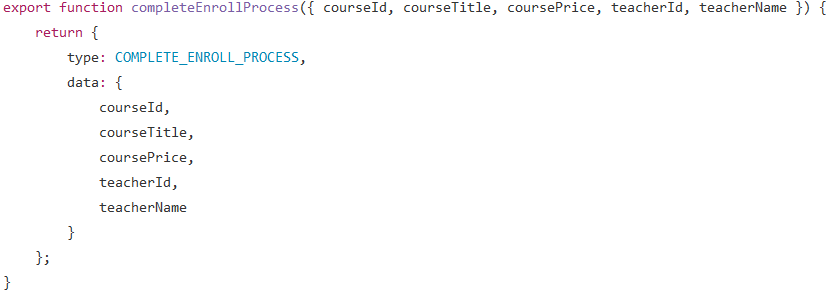
\includegraphics[scale=0.8]{figure/enroll.png}
    \caption{The action creator called when a user books a course.}
    \label{fig:enroll}
\end{figure}

This function is a Redux action creator: it returns a Redux action, containing a type (\guillemotleft{} COMPLETE\_ENROLL\_PROCESS \guillemotright{}) and some data (course id, teacher id\ldots). The action is then mapped to the analytics by the \textit{mapActionsToAnalytics} function, visible on {\sc figure}~\ref{fig:mapActions}.

\begin{figure}[H]
    \centering
    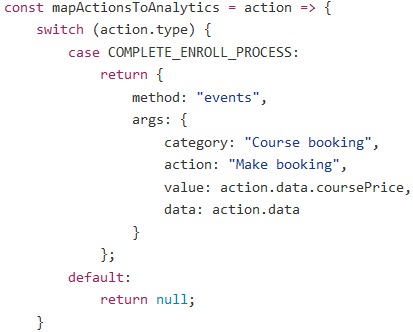
\includegraphics[scale=0.8]{figure/mapActions.png}
    \caption{The function mapping Redux actions to analytics.}
    \label{fig:mapActions}
\end{figure}

The returned object contains two fields, the method (always \guillemotleft{} events \guillemotright{} no matter the action) and the args. The args represent the data needed for the analytics, that will be displayed and analyzed by two tools: 

\textbf{Google Analytics} offering numerous services: calculation of conversion rates, estimation of sales, information on used devices\ldots Plus, it provides help for marketing and advertising~\cite{googleAnalytics}. 

\textbf{Mixpanel} focusing on funnels, i.e. visual representations of how users move through a series of events. This aims at finding out where users abandon and why~\cite{mixpanel}.

Now that the main techniques and technologies have been introduced, {\sc section}~\ref{sec:accomplish} presents the most important achievements of the traineeship.